\chapter{Requirement specification}
\label{kravsspec}
The following chapter contains a general description of \textit{FingerDrums}, a description of the use case for the product and finally a simple requirement specification will be presented.

%I dette kapitel opstilles en projektplan med en generel produktbeskrivelse og specifikke systemkrav. Projektplanen, produktbeskrivelsen og systemkravene formuleres for at produktet i sidste ende kommer til at fungere efter hensigten. Produktet beskrives først generelt ved hjælp af Use Cases. På baggrund af den generelle produktbeskrivelse formuleres en række specifikke systemkrav. De endelige krav vil til sidst opsummeres i prioriteret rækkefølge. 

\section{General description}
%Målet for projektet er at udarbejder et elektronisk instrument, som kan simulere lyde fra et trommesæt. De forskellige trommelyde afspilles ved hjælp af fingerspidserne, hvor hver fingerspids har sin egen unikke lyd. En lyd afspilles når en finger laver en trommebevægelse. En trommebevægelse er en gestikulering hvor fingerspidsen rammer en overflade og derved møder modstand. Modstanden detekteres af en elektronisk sensor. En trommebevægelse kan derved laves på mange forskellige overflader, eksempelvist et bord, en væg eller et lårben. Brugeren af produktet vælger med fingerspidsernes sensorer hvilken lyd der skal afspilles og hvornår den skal afspilles.
%
%Trommelydende kan i princippet varieres og skiftet ud efter brugerens ønske. Som udgangspunkt kan en unik lyd for hver fingerspids frembringes. Brugeren kan ved hjælp af et display udskifte eller omarrangere de unikke lyde efter behov. På den måde kan produktet tilpasses specifikke brugere samt brugssituationer. Brugeren kan ændre lydstyrken ved hjælp af displayet. Det er også ved hjælp af displayet at produktets tænd/sluk funktion tilgås. 

The \textit{FingerDrums} should be integrated into a glove which holds the sensors in place. For this prototype the sensors in the fingers of the glove are wired to an Arduino which communicates with a PC. The PC then plays the sounds. No interface is integrated on the glove in this iteration, however, ideally an interface should be integrated on the wrist of the glove allowing the user to change the sound profile, volume etc.

\section{Use Cases}
\label{UseCase}
Here the basic functional requirements will be listed in a Use Case diagram which explains the actors on the system and how they are correlated between each other.
%Følgende afsnit fokusere på de funktionelle krav som produktet skal opfylde. Produktets funktioner beskrives ved hjælp af Use Cases, hvor grænseflader mellem aktører og funktioner vil fremgå. Den generelle produktbeskrivelse lægger op til uddybelse af produktets funktionelle krav, samt en opdeling af de aktører, som indgår i processen.
In order for the \textit{FingerDrums} concept to work the user should be able to play sounds, change which sounds should be played, change the volume and turn the system on/off. As mentioned at the top in \autoref{Ideation} the purpose is to develop an electrical prototype which allows to play drum sounds and perhaps contain a display. On \autoref{fig:protoUseCase} the Use Case diagram is shown. The internal actors are denoted Display, Sensors, and Control System. 

%Brugeren af produktet skal have mulighed for at afspille lyde, udskifte lyde, ændre lydstyrke samt tænde og slukke for systemet. Afspil lyd, Udskift lyd, Ændr lydstyrke og Tænd/sluk er derfor essentielle funktioner at implementere, for at produktet fungere optimalt. For at brugeren i sidste ende kan tilgå funktionerne er det nødvendigt at kende de interne og eksterne aktører som er involveret i  processerne. Som nævnt i ***section - Generel produktbeskrivelse*** er målet for projektet at fremstille en elektronisk prototype, som ved hjælp af et styresystem kan afspille forskellige trommelyde på baggrund af brugerens interaktion med sensorer og et display. De interne aktører; Sensorer, Display og Styresystem, symboliserer hvor der foregår en interaktion mellem produktets forskellige funktioner og aktører. Brugeren selv defineres som en ekstern aktør, ligsom højtaler, der i sidste ende afspiller lyden, også fremgår som eksterne aktører. Det sker for at simplificere Use Case diagrammet til kun at omfatte systemet selv. Use Case diagrammet på \autoref{fig:protoUseCase} fokusere derfor på de interne aktører, som gør funktionerne tilgængelige via grænsefladerne mellem funktion og aktør. 

\begin{figure}[htbp]
\centering
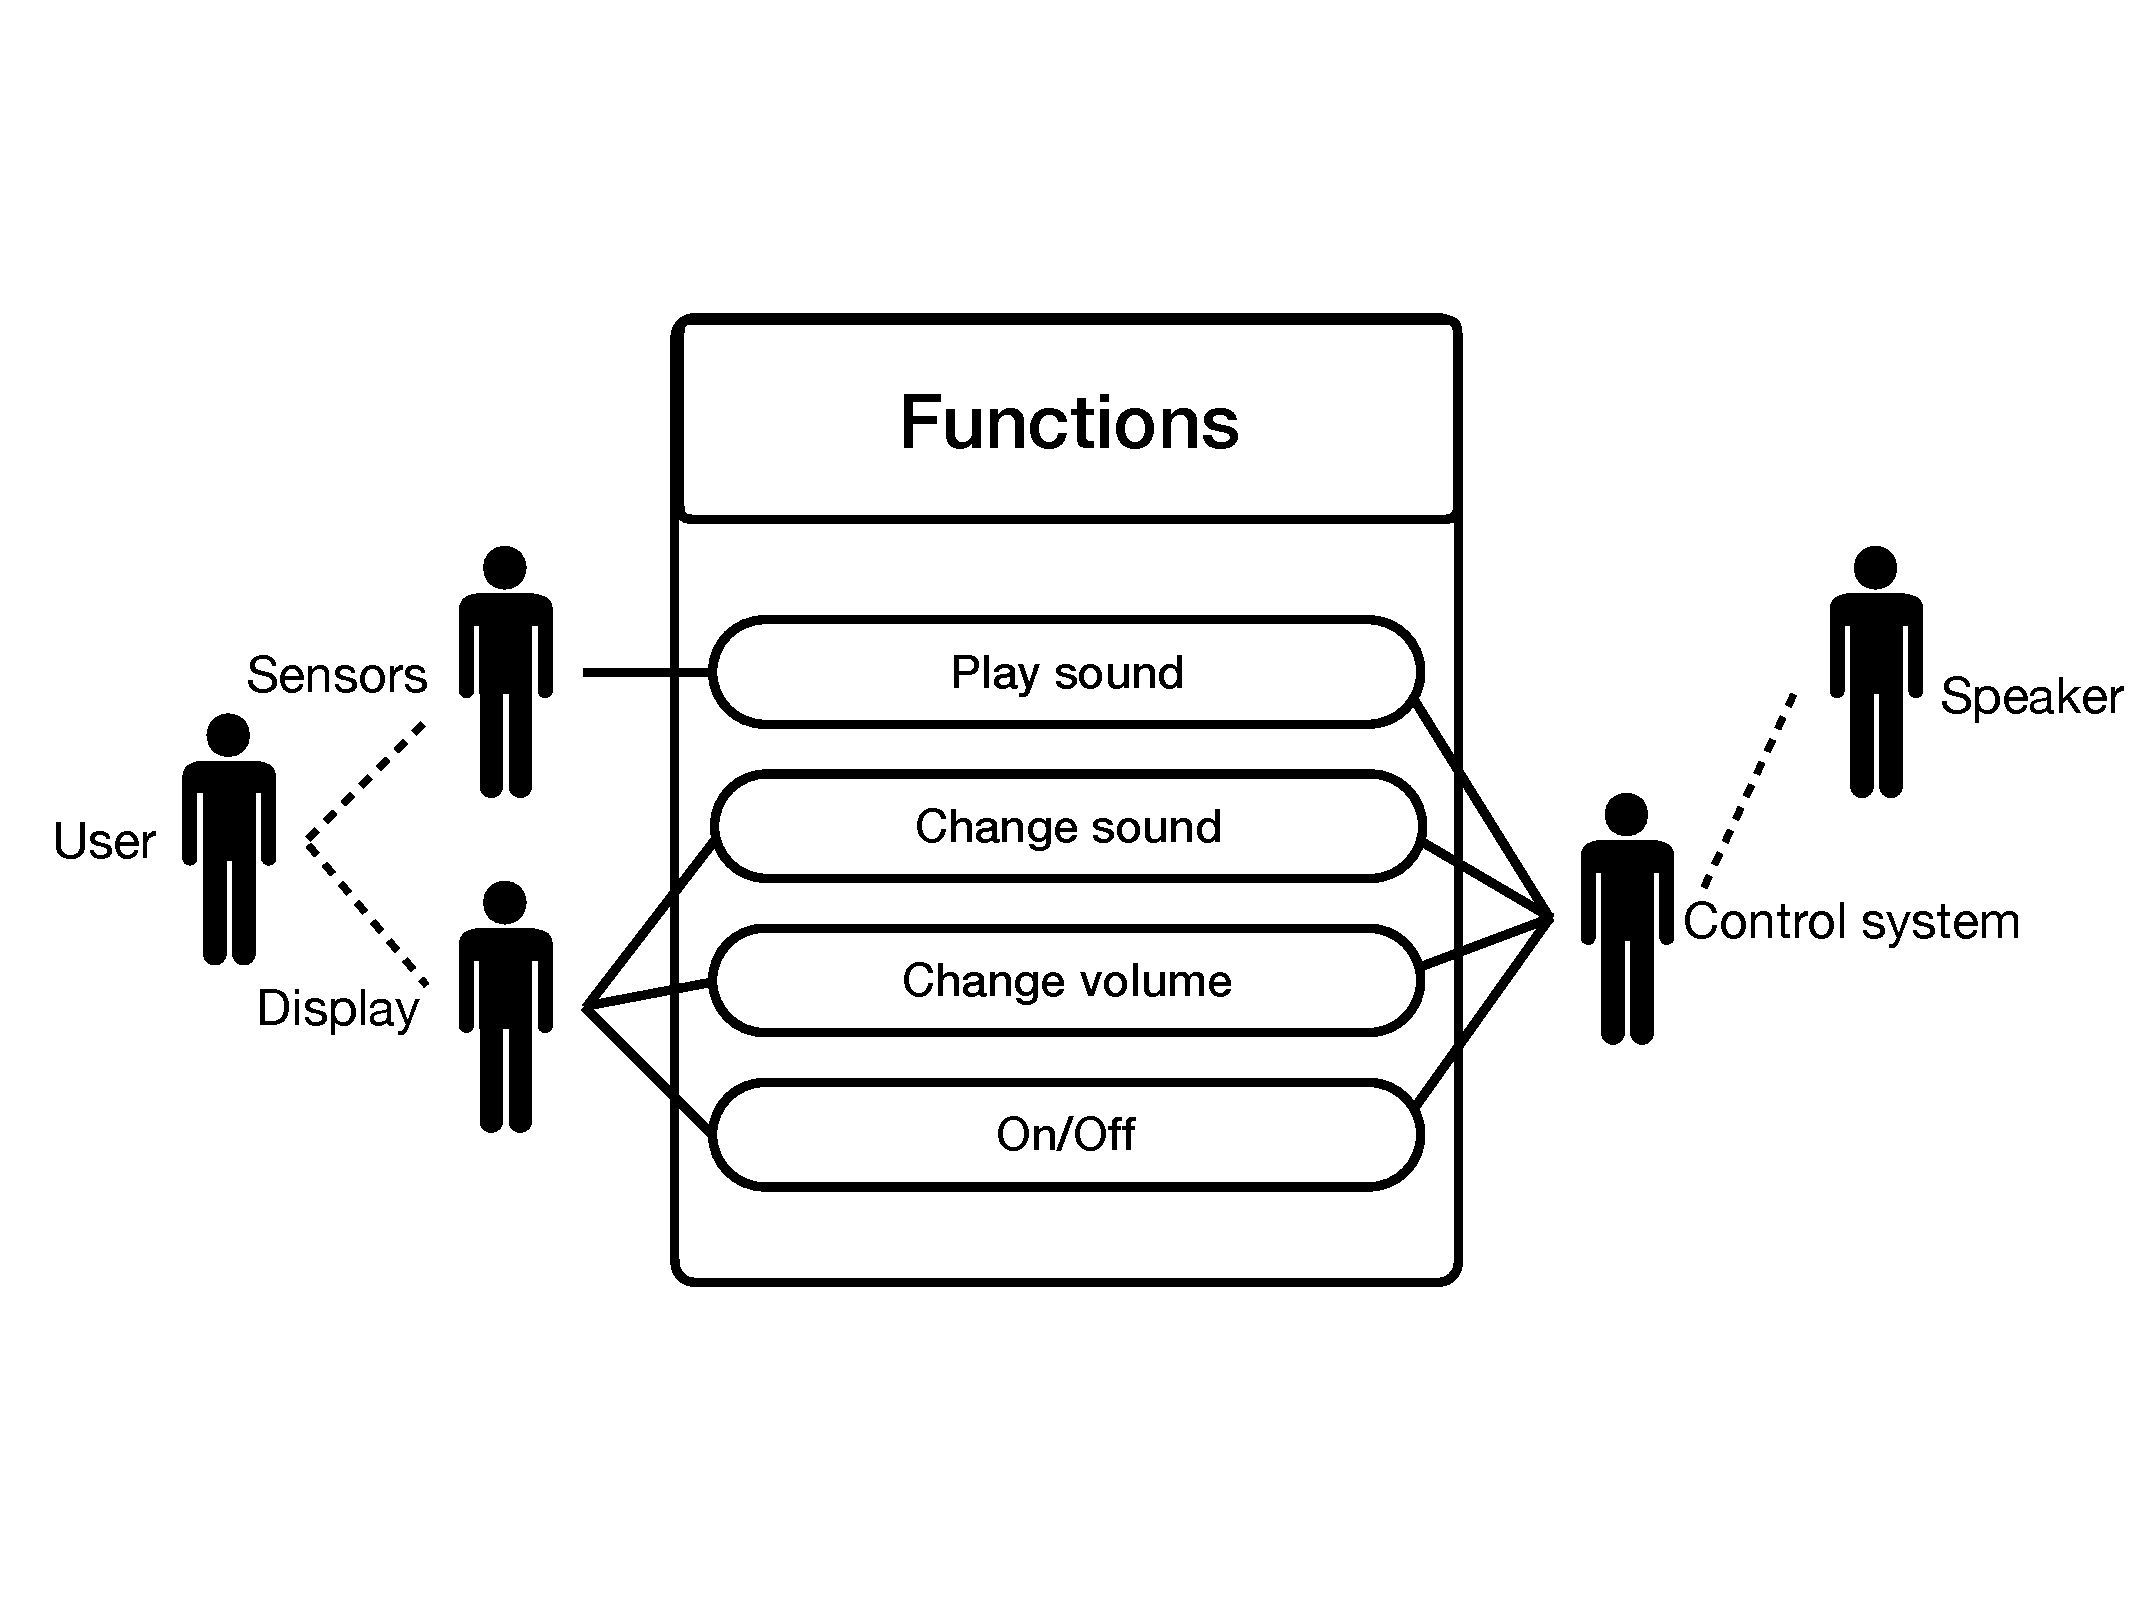
\includegraphics[scale=0.4]{Figure/protoUseCase01.pdf}
\caption{
Use Case diagram for the complete system. The four Use Cases are connected to their respective actors. The interface is located between the use case and the actor.}
\label{fig:protoUseCase}
\end{figure}

\subsection{Play sound}
The user interacts with a sensor in order to play a unique drum sound. The sensor signals, via the interface, to the system that the user performed a drum motion. the system reacts by sending a signal to the speaker which plays a sound.
%Brugeren interagere med sensorerne for at afspille en unik trommelyd. Sensorerne signalere, via grænsefladen til styresystemet, at en finger laver en trommebevægelse. Styresystemet reagere på signalet og interagere med den eksterne aktør, højtaler, der derefter afspiller lyden.    

\subsection{Change sound}
the user interacts with the display in order to change or rearrange a sound. The display signals the system to change a sound, and does so via the interface. The system reacts by changing the sound in question.
%Brugeren interagere med displayet for at udskifte eller omarrangere en lyd. Displayet signalere, via grænsefladen til styresystemet, at en lyd skal ændres. Styresystemet reagere på signalet og ændre derefter den respektive lyd.   

\subsection{Change volume}
The user interacts with the display in order to change volume. The display signals the system via the interface, and the system changes the volume accordingly.
%Brugeren interagere med displayet for at ændre lydstyrken. Displayet signalere, via grænsefladen til styresystemet, at lydstyrken skal ændres. Styresystemet reagere på signalet og ændre derefter lydstyrken. 

\subsection{On/Off}
The user interacts with the display to turn on or off the system. The display signals the system after which the system reacts by turning on or off respectively. 
%Brugeren interagere med displayet for at tænde eller slukke systemet. Displayet signalere, via grænsefladen til styresystemet, at systemet enten skal tændes eller slukkes. Styresystemet reagere på signalet, hvorefter systemet enten tænder eller slukker

\section{Specific requirements}
The following section contains a description of the specific requirements for the prototype. First the requirements regarding functionality will be described, followed by requirements to the internal actors and finally any general requirements, with respect to design and quality, regarding the overall system.
%Følgende afsnit giver en detaljeret beskrivelse af de specifikke krav der måtte være til produktet. Først beskrives kravende til funktionaliteten, derefter kravende til de interne aktører og til sidst beskrives kravende til det samlede system, herunder kvalitetskrav og designkrav. 

\subsection{Functionality Requirements}
\label{Krav_til_funktionalitet}
As this prototype is mainly meant to be a proof of concept, the most important functional requirement is that the prototype can play the correct drum sound when the user performs a drum motion with their finger. This means playing a specific sound according to the finger that was used to make the drum motion, which activated the sensor. The sound has to be played immediately after the drum motion is performed and in the first iteration of the prototype there has to be some form of drum sound, meaning a complex sound ie. not a simple sinus tone. The sound should only be played once per drum motion. This means if the user presses their finger against a surface for a longer period of time keeping the sensor active, the sound should still only be played once until the user lifts the sensor allowing the sensor to go back to zero. The system should also be able to play all five sounds simultaneously in the event that the user activates more than one sensor at the same time.\\
Changing volume, sound profile, and turning the system on/off from the display as described in \autoref{UseCase} are not a priority requirement and should simply be simulated by the PC in the first iteration of the prototype.

%Som det fremgår af afsnit ***HENVISNING ÚSE CASES***, skal fire funktioner implementeres. Funktionerne initieres via aktørerne Sensor og Display. Aktørerne virker som brugerinterface, og er dermed brugerens mulighed for at interagere med aktøren Styresystem. Selve funktionerne eksekveres af aktøren Styresystem.

%Ved funktionen, Afspil lyd, menes muligheden for at afspille en specifik lydfil ækvivalent til den sensor brugeren interagere med. Lydfilen skal som udgangspunkt imitere en lyd fra et trommesæt. Lyden forventes derfor at bestå af et kompleks signal frem for en ren sinustone. Lyden afspilles umiddelbart efter brugeren har interageret med en sensor, uden mærkbar forsinkelse. En mærkbar forsinkelse defineres som en forsinkelse hvor auditive feedback afspilles tilpas lang tid efter interaktionen med sensoren til at brugeren kan detektere en forsinkelse. Lyden afspilles en enkelt gang ved hver interaktion med en sensor. Hvis brugeren interagere med flere sensorer samtidigt afspilles de respektive lyde samtidig.  

%Ved funktionen, Udskift lyd, menes muligheden for at udskifte de specifikke trommelyde. Derved har brugeren mulighed for at udskifter og omarrangere de lyde der frembringes ved at intergere med en sensor. Lydene udskiftes ved at interagere med aktøren display, hvorefter styresystemet ændre de respektive lyde. 

%Ved funktionen, Ændr lydstyrke, menes muligheden for at skrue op og ned for lydstyrken af trommelydene. Derved kan brugeren dimensionere lydniveauet så det passe til omgivelserne. Lydstyrken ændres ved at interagere med aktøren display, hvorefter styresystemet ændre lydstyrken.

%Ved funktionen, Tænd/Sluk, menes muligheden for at tænde eller slukke for systemet. Derved har brugeren mulighed at vælge hvornår systemet er aktivt og afspiller lyde ved interaktion med sensorerne.

\subsection{Requirements of internal actors}
The main internal actors in the system are the sensors situated at the end of each finger of the glove. These sensors should be able to detect when the user hits their finger against any surface but should not react from just being in motion alone, but should require contact of a force being applied directly to it. \\
Other internal actors include the display and speaker, but these actors are not being prioritized in this iteration of the prototype and will simply be simulated by the PC.

\subsection{General requirements}
General requirements include the sensors being mounted into the fingers of a glove that can be worn and used as intended. The design should be sturdy enough to be used without the sensors coming loose and should generally be usable as a musical instrument.
%\begin{enumerate}
%\item[\textbf{§}] \textbf{1} Afspil lyd 
%\item[\textbf{§}] \textbf{2} Udskift lyd
%\item[\textbf{§}] \textbf{3} Ændr lydstyrke
%\item[\textbf{§}] \textbf{4} Tænd/Sluk
%\end{enumerate}
%\subsection{Krav til aktører}
%\subsection{krav til samlet system}


 



%Hovedfunktioner: 
%Begrænsninger:
%Brugerprofiler:

%Specifikke krav: 
%Sensorene skal kunne signalere om en respektiv finger trommer eller ej. 
%Styringsenheden skal kunne aflæse signalet fra sensorerne, behandler signalet og afspille en lydfil til en højtaler.

%… detailkrav/
%ydelseskrav/
%kvalitetskrav/
%designkrav/ - flexibel let handske      

 
